\documentclass[a4paper,12pt]{article}

\title{Data Privacy Homework 1}
\author{Daoyu Wang   PB21030794}
\date{November 7}
\usepackage{color}
\usepackage{graphicx}
\usepackage{amsmath}
\usepackage{algorithm}
\usepackage{algorithmicx}
\usepackage{indentfirst}
\usepackage{algpseudocode}
\usepackage{fancyhdr} 
\usepackage[table]{xcolor}
\pagestyle{fancy}
% 页眉设置
\fancyhead[L]{Data Privacy Homework 1}
\fancyhead[R]{Daoyu Wang}
% \fancyhead[C]{}
% 页脚设置
% \fancyfoot[L]{left root}
% \fancyfoot[C]{\thepage}
% \fancyfoot[R]{right root}
\setlength{\headheight}{14.49998pt}
\addtolength{\topmargin}{-2.49998pt}


\begin{document}
\maketitle
\pagenumbering{roman}
\tableofcontents
\newpage

\section{K-anonymity}

\subsection{(a)}
The quasi-identifier attributes are \textbf{Zip Code}, \textbf{Age}, \textbf{Salary}, \textbf{Nationality}.

\subsection{(b)}
Assume \textbf{H} represents \textbf{Heart Disease}, \textbf{V} represents \textbf{Viral Infection}, \textbf{C} represents \textbf{Cancer}.

Assume \textbf{R} represents \textbf{Russian}, \textbf{A} represents \textbf{American}, \textbf{C} represents \textbf{Chinese}, \textbf{I} represents \textbf{Indian}, \textbf{J} represents \textbf{Japanese}.

\subsubsection{generalization hierarchies}
When $k = 2$, the generalization hierarchies are as follows:

\begin{figure}[ht]
    \centering
    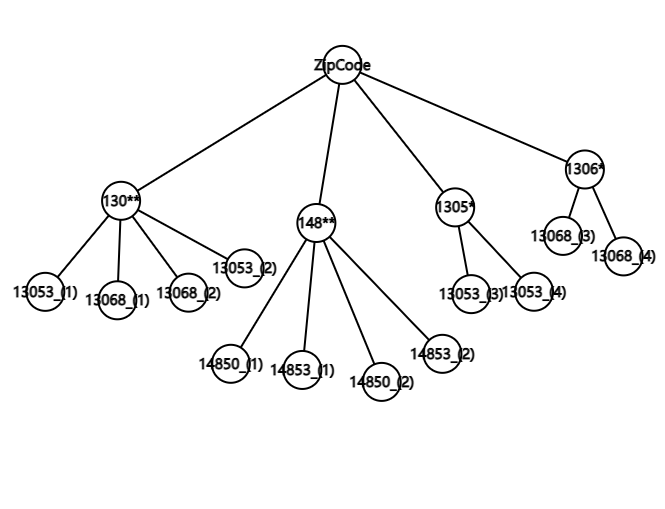
\includegraphics[width=0.45\textwidth]{assets/3.png}
    \hfill
    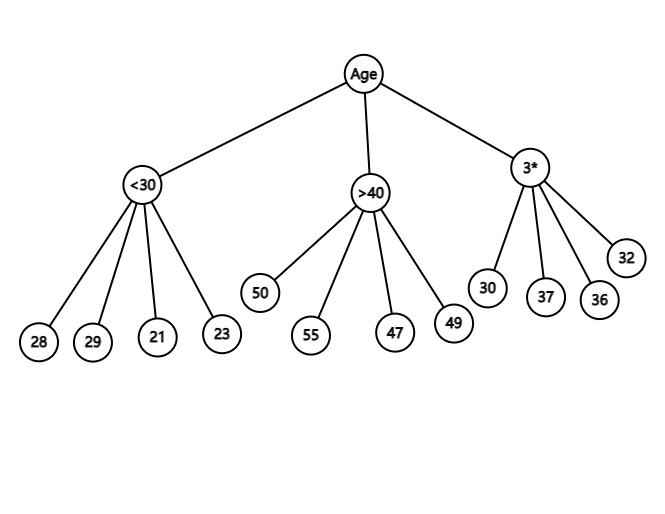
\includegraphics[width=0.45\textwidth]{assets/4.png}
    \caption{generalization hierarchies: Zip Code, Age}
\end{figure}

\newpage

\begin{figure}[ht]
    \centering
    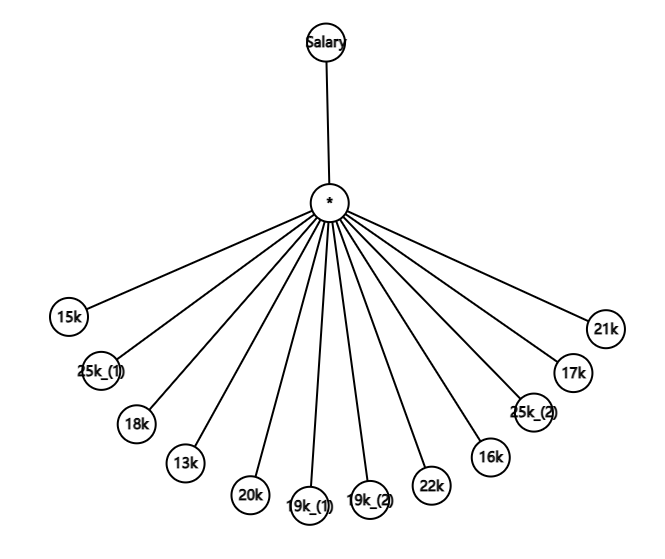
\includegraphics[width=0.45\textwidth]{assets/6.png}
    \hfill
    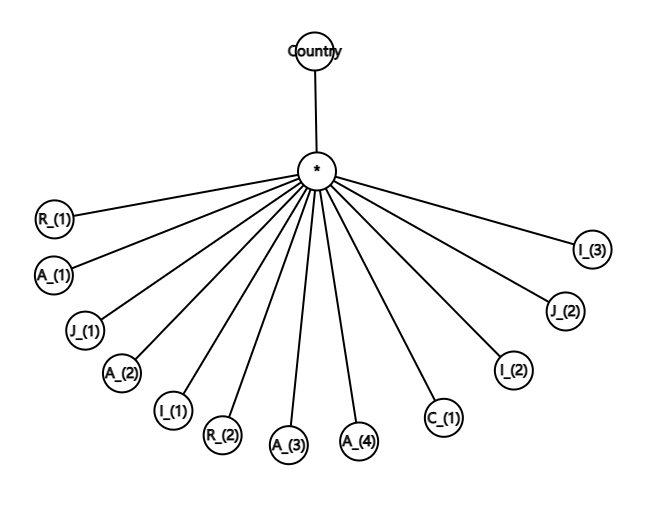
\includegraphics[width=0.45\textwidth]{assets/5.png}
    \caption{generalization hierarchies: Salary, Nationality}
\end{figure}

\subsubsection{released table}
The released table is as follows:

\begin{table}[!ht]
    \centering
    \begin{tabular}{|l|l|l|l|l|l|}
        \hline
        \textbf{}   & \textbf{Zip Code} & \textbf{Age} & \textbf{Salary} & \textbf{Nationality} & \textbf{Condition} \\ \hline
        \rowcolor{green!60}
        \textbf{1}  & 130**             & < 30         & *               & *                    & H                  \\ \hline
        \rowcolor{green!60}
        \textbf{2}  & 130**             & < 30         & *               & *                    & H                  \\ \hline
        \rowcolor{green!60}
        \textbf{3}  & 130**             & < 30         & *               & *                    & V                  \\ \hline
        \rowcolor{green!60}
        \textbf{4}  & 130**             & < 30         & *               & *                    & V                  \\ \hline
        \rowcolor{blue!60}
        \textbf{5}  & 1485*             & > 40         & *               & *                    & C                  \\ \hline
        \rowcolor{blue!60}
        \textbf{6}  & 1485*             & > 40         & *               & *                    & H                  \\ \hline
        \rowcolor{blue!60}
        \textbf{7}  & 1485*             & > 40         & *               & *                    & V                  \\ \hline
        \rowcolor{blue!60}
        \textbf{8}  & 1485*             & > 40         & *               & *                    & V                  \\ \hline
        \rowcolor{yellow!60}
        \textbf{9}  & 1305*             & 3*           & *               & *                    & C                  \\ \hline
        \rowcolor{yellow!60}
        \textbf{10} & 1305*             & 3*           & *               & *                    & C                  \\ \hline
        \rowcolor{red!60}
        \textbf{11} & 1306*             & 3*           & *               & *                    & C                  \\ \hline
        \rowcolor{red!60}
        \textbf{12} & 1306*             & 3*           & *               & *                    & C                  \\ \hline
    \end{tabular}
\end{table}

\subsubsection{loss metric}
For a tuple $t$, suppose the value of $t[A]$ has been generalized to $x$.
Letting $|A|$ represent the total number of leaf nodes in the tree;
letting $M$ represent the number of leaf nodes in the subtree rooted at $x$,
then the loss for $t[A]$ is $\frac{M - 1}{|A| - 1}$.

The loss for attribute $A$ is the average of the loss for all tuples $t$. The
\textbf{LM} for the entire data set is the sum of the losses for each attribute.
The loss metric is as follows:

\begin{itemize}
    \item \textbf{Zip Code:} $|A| = 16$
          \begin{itemize}
              \item \textbf{130**:} $M = 4$, $loss = \frac{4 - 1}{16 - 1} = \frac{1}{5}$
              \item \textbf{148**:} $M = 4$, $M = 4$, $loss = \frac{4 - 1}{16 - 1} = \frac{1}{5}$
              \item \textbf{1305*:} $M = 2$, $M = 2$, $loss = \frac{2 - 1}{16 - 1} = \frac{1}{15}$
              \item \textbf{1306*:} $M = 2$, $M = 2$, $loss = \frac{2 - 1}{16 - 1} = \frac{1}{15}$
          \end{itemize}
          loss of \textbf{Zip Code} is $\frac{\frac{1}{5} + \frac{1}{5} + \frac{1}{15} + \frac{1}{15}}{4} = \frac{2}{15}$.
    \item \textbf{Age:} $|A| = 15$
          \begin{itemize}
              \item \textbf{<30:} $M = 4$, $loss = \frac{4 - 1}{15 - 1} = \frac{3}{14}$
              \item \textbf{>40:} $M = 4$, $loss = \frac{4 - 1}{15 - 1} = \frac{3}{14}$
              \item \textbf{3*:} $M = 4$, $loss = \frac{4 - 1}{15 - 1} = \frac{3}{14}$
          \end{itemize}
          loss of \textbf{Age} is $\frac{\frac{3}{14} + \frac{3}{14} + \frac{3}{14}}{3} = \frac{3}{14}$.
    \item \textbf{Salary:} $|A| = 13$
          \begin{itemize}
              \item \textbf{*:} $M = 12$, $loss = \frac{12 - 1}{13 - 1} = \frac{11}{12}$
          \end{itemize}
          loss of \textbf{Salary} is $\frac{11}{12}$.
    \item \textbf{Nationality:} $|A| = 13$
          \begin{itemize}
              \item \textbf{*:} $M = 12$, $loss = \frac{12 - 1}{13 - 1} = \frac{11}{12}$
          \end{itemize}
          loss of \textbf{Nationality} is $\frac{11}{12}$.
\end{itemize}

So the \textbf{LM} for the entire data set is the sum of the losses for each attribute: $\frac{2}{15} + \frac{3}{14} + \frac{11}{12} + \frac{11}{12} \approx 2.181$.

\section{L-Diversity}
\subsection{(a)}
If the attributes meet recursive (2,2)-diversity, they should meet the following formula:
\begin{equation}
    r_1 < 2(r_2+r_3+\cdots+r_m)
\end{equation}
Firstly, we should count the frequency of each attribute value in each group:

\paragraph*{Group1}
\begin{equation}
    \begin{aligned}
        n(q^*, Heart\space Disease)   & = 1/4 \\
        n(q^*, Viral\space Infection) & = 1/4 \\
        n(q^*, Cancer)                & = 2/4 \\
    \end{aligned}
\end{equation}

\paragraph*{Group2}
\begin{equation}
    \begin{aligned}
        n(q^*, Heart\space Disease)   & = 1/4 \\
        n(q^*, Viral\space Infection) & = 2/4 \\
        n(q^*, Cancer)                & = 1/4 \\
    \end{aligned}
\end{equation}

\paragraph*{Group3}
\begin{equation}
    \begin{aligned}
        n(q^*, Heart\space Disease)   & = 1/4 \\
        n(q^*, Viral\space Infection) & = 1/4 \\
        n(q^*, Cancer)                & = 2/4 \\
    \end{aligned}
\end{equation}

We can find that:$\frac{2}{4} < 2(\frac{1}{4}+\frac{1}{4})$, and this is suitable for each group.
So the attributes meet recursive (2,2)-diversity.

\subsection{(b)}
First we can define the entropy of l-diversity:
Assume that the sequence of l-diversity in table $T$ is $L = {l_1, l_2 ,\cdots, l_m}$:
\begin{equation}
    H = \sum\limits_{i=1}^m -l_i\log_2 l_i
\end{equation}
After generalization, the sequence of l-diversity is $L' = {l'_1, l'_2 ,\cdots, l'_m}$ in table $T^*$:
Assume that some items in $L$ are merged, and the merged item in $L'$ is $l_i$:
Assume the items in $L$ is $l_{j_1}, l_{j_2}, \cdots l_{j_k}$.
Obviously, due to repeated sensitive information, the item $l_i$ after merging
is not as large as the sum of items before merging, as $l_i < \sum\limits_{r=1}^{k} l_{j_r}$.

For the function $f(x) = -x\log_2 x$, it can be proved that it is a convex function. Anyway, it has a property that:
\begin{equation}
    f(\sum\limits_{i=1}^{n} x_i) > \sum\limits_{i=1}^{n} f(x_i)
\end{equation}
So:
\begin{equation}
    f(\sum\limits_{r=1}^{k} l_{j_r}) > \sum\limits_{r=1}^{k} f(l_{j_r})
\end{equation}
Then, when analysing l-diversity, the parameter $l$ is larger than $1$.
Meanwhile, when $x > 1$, the function $f(x)$ is a decreasing function, so:
\begin{equation}
    f(l_i) > f(\sum\limits_{r=1}^{k} l_{j_r})
\end{equation}
Combining the above two inequalities formula $(7)$ and $(8)$, we can get:
\begin{equation}
    f(l_i) > \sum\limits_{r=1}^{k} f(l_{j_r})
\end{equation}
So, after merging, the entropy is larger than before merging which means $T^*$ also satifies entropy l-diversity.

\section{T-closeness}
\subsection{(a)}
Numerical attribute values are ordered. Let the attribute
domain be ${v_1, v_2, \cdots, v_m}$ and assume $v_i$ is the $i^{th}$ smallest value.

To calculate the EMD under ordered distance,
we only need to consider the flow of mass transfer between adjacent elements,
as any transfer between two more distant elements can be effectively decomposed into multiple transfers between adjacent elements.
According to this conclusion, the minimum workflow $f_{ij}$ can be achieved by sequentially satisfying all elements of Q.
We can first consider \textbf{element 1} greedily, which has an extra amount of $p_1 - q_1$.
Assume, without loss of generality, which represents that $p_1 - q_1 < 0$,
an amount of $q_1 - p_1$ should be transported from other elements to \textbf{element 1} to make up for this increase.
We can surely transport this from \textbf{element 2}.
After this transportation, \textbf{element 1} is satisfied and \textbf{element 2} has an extra amount of
$(p_1 - q_1) + (p_2 - q_2)$.
Similarly, we can satisfy \textbf{element 2} by transporting an amount of $(p_1 - q_1) + (p_2 - q_2)$ between \textbf{element 2} and \textbf{element 3}.
This process continues until element m is satisfied and Q is reached.

It should be noted that due to the two opposite cases ($(p_1 - q_1) + (p_2 - q_2) + \cdots + (p_i - q_i) > 0$ or $ < 0$), the absolute value must be added when calculating each flow.

Formally, let $r_i = p_i - q_i ,(i=1,2,...,m)$, then the distance
between P and Q can be calculated as:
\begin{equation}
    \begin{aligned}
        D[\textbf{P}, \textbf{Q}] & = \frac{1}{m-1}(|r_1| + |r_1+ r_2| + \cdots + |r_1 + r_2 + \cdots + r_{m-1}|) \\
                                  & =\frac{1}{m-1}\sum\limits_{i = 1}^{m}|\sum\limits_{j = 1}^{j=i} r_i|
    \end{aligned}
\end{equation}

\subsection{(b)}
Assume that $Q$ is the sequence of salary.
Obviously, $Q = \{3k, 4k, 5k, 6k,$
\newline
$7k, 8k, 9k, 10k, 11k\}$ which is ordered.
The salary sequence corresponding to three groups are:
$P_1 = \{4k, 5k, 6k\}$, $P_2 = \{3k, 8k, 11k\}$,  $P_3 = \{7k, 9k, 10k\}$.

To calculate the EMD under ordered distance, we should search for the optimized flow between $P_i$ and $Q$
Tne optimal mass flow that transforms P1 to Q is to move 1/9 probability mass across the following pairs:
\begin{equation}
    \begin{aligned}
         & (4k \rightarrow 3k), (4k \rightarrow 4k), (4k \rightarrow 5k)   \\
         & (5k \rightarrow 6k), (5k \rightarrow 7k), (5k \rightarrow 8k)   \\
         & (6k \rightarrow 9k), (6k \rightarrow 10k), (6k \rightarrow 11k)
    \end{aligned}
\end{equation}
The cost of this flow is: $\frac{1}{9}\times(1+0+1+1+2+3+3+4+5)/(9-1) = 0.278$

Similarly, the cost of the optimal flow that transforms $P2$ to $Q$ is: $\frac{1}{9}\times(0+1+2+2+1+0+2+1+0)/(9-1) = 0.125$.
the cost of the optimal flow that transforms $P3$ to $Q$ is: $\frac{1}{9}\times(4+3+2+3+2+1+1+0+1)/(9-1) = 0.236$.

According to three results, we can get the t-closeness of this table is $0.278$. In other word, this table is 0.278-closeness.

\section{Prior and posterior}
\subsection{(a)}
Above all, to simplify the expression, we can reduce formula $P(R(x) = 0 | x = k)$ to $P(R(k) = 0)$.

\subsubsection{$x = 0$ (given $R_1(x) = 0$)}
The prior and posterior probability of $x = 0$ (given $R_1(x) = 0$) is as follows:

By Bayesian formula and assume $P_1 = P(x = 0 | R_1(x) = 0)$:
\begin{equation}
    \begin{aligned}
        P_1 & = \frac{P(R_1(0) = 0)\cdot P(x = 0)}{P(R_1(0) = 0)\cdot P(x = 0) + \sum\limits_{k = 1}^{100}P(R_1(k) = 0)\cdot P(x = k)}                                                \\
            & = \frac{(30\% + 70\%\times \frac{1}{101}) \times 0.01}{(30\% + 70\%\times \frac{1}{101}) \times 0.01 + \sum\limits_{k = 1}^{100} 70\%\times \frac{1}{101} \times 0.099} \\
            & = 30.9\%
    \end{aligned}
\end{equation}

\subsubsection{$x = 0$ (given $R_3(x) = 0$)}
The prior and posterior probability of $x = 0$ (given $R_3(x) = 0$) is as follows:

Firstly, we can easily get the probability of $R_2(x) = 0$ when $x = k$:
\begin{equation}
    \begin{aligned}
        P(R_2(k) = 0) & = P((k + \xi)mod(101))                                              \\
                      & = \begin{cases}
                              P(k + \xi = 0) = 0                     & \quad 11\leq k \leq 90   \\
                              P((k + \xi)mod(101)= 0) = \frac{1}{21} & \quad 0 \leq k \leq 10   \\
                              P((k + \xi)mod(101)= 0) = \frac{1}{21} & \quad 91 \leq k \leq 100
                          \end{cases}
    \end{aligned}
\end{equation}

By Bayesian formula and assume $P_3 = P(x = 0 | R_3(x) = 0)$:
\begin{equation}
    \begin{aligned}
        P_3 & = \frac{P(R_3(0) = 0)\cdot P(x = 0)}{P(R_3(0) = 0)\cdot P(x = 0) + \sum\limits_{k = 1}^{100}P(R_3(k) = 0)\cdot P(x = k)} \\
            & = \frac{P(R_3(0) = 0)}{P(R_3(0) = 0) + \sum\limits_{k = 1}^{100}P(R_3(k) = 0)\cdot 0.99}
    \end{aligned}
\end{equation}
Among this formula:
\begin{equation}
    \begin{aligned}
        P(R_3(0) = 0) & = 50\% \cdot P(R_2(0) = 0) + 50\%\times \frac{1}{101}  \\
                      & = 50\% \times \frac{1}{21} + 50\% \times \frac{1}{101}
    \end{aligned}
\end{equation}
\begin{equation}
    \begin{aligned}
        P(R_3(k) = 0) & = 50\% \cdot P(R_2(k) = 0) + 50\%\times \frac{1}{101} \\
                      & =
        \begin{cases}
            50\% \times \frac{1}{21} + 50\% \times \frac{1}{101} & \quad 0 \leq k \leq 10   \\
            50\% \times \frac{1}{21} + 50\% \times \frac{1}{101} & \quad 91 \leq k \leq 100 \\
            50\% \times \frac{1}{101}                            & \quad 11 \leq k \leq 90
        \end{cases}
    \end{aligned}
\end{equation}
Substitute into formula $(14)$:
\begin{equation}
    P_3  = 2.9\%
\end{equation}

\subsubsection{$x\in [20, 80]$ (given $R_2(x) = 0$)}
The prior and posterior probability of $x = i \in [20, 80]$ (given $R_2(x) = 0$) is as follows:

By Bayesian formula and assume $P_2 = P(x = i | R_2(x) = 0)$:
\begin{equation}
    \begin{aligned}
        P_2 & = \frac{P(R_2(x) = 0 | x = i)\cdot P(x = i)}{P(R_2(0) = 0)\cdot P(x = 0) + \sum\limits_{k = 1}^{100}P(R_2(k) = 0)\cdot P(x = k)} \\
            & = 0
    \end{aligned}
\end{equation}

\subsection{(b)}
$R_3$ is more suitable, the probability distribution is not as biased as $R_1$ (as $P(x = 0 | R_1(x) = 0)$ is $70\%$, so large that is easy to guess), nor is the data range as small as $R_2$.
\newpage
\section{K-anonymity in graphs}
\subsection{(a)}
Connect an edge between \textbf{Bob} and \textbf{Lucy}, like this:
\begin{figure}[ht]
    \centering
    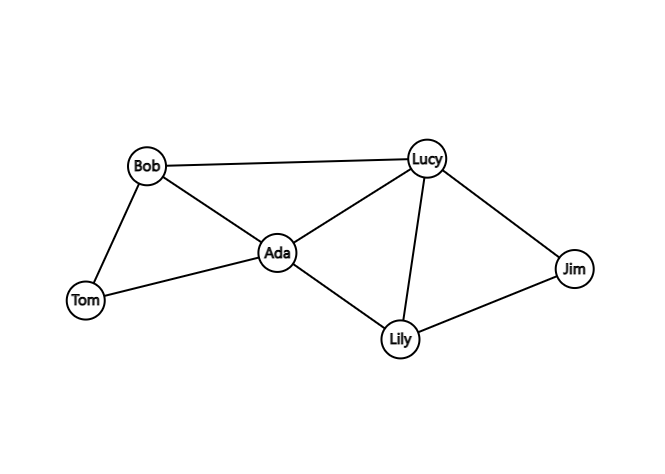
\includegraphics[width=0.8\textwidth]{assets/1.png}
    \caption{2-Anonymous Graph}
\end{figure}
the degree sequence of the graph is $\{2, 3, 4, 4, 3, 2\}$ which is 2-anonymous.
\subsection{(b)}
Because the total degree will increase by 2 because of an additional edge, and the total degree is now 16.
So assuming that the final degree sequence consists of three $a$ and three $b$, then $3(a + b)$ is an even number, that is,
$a + b$ is an even number, taking $a$ as $4$ and $b$ as $6$, the result is as shown in the figure below:
\begin{figure}[ht]
    \centering
    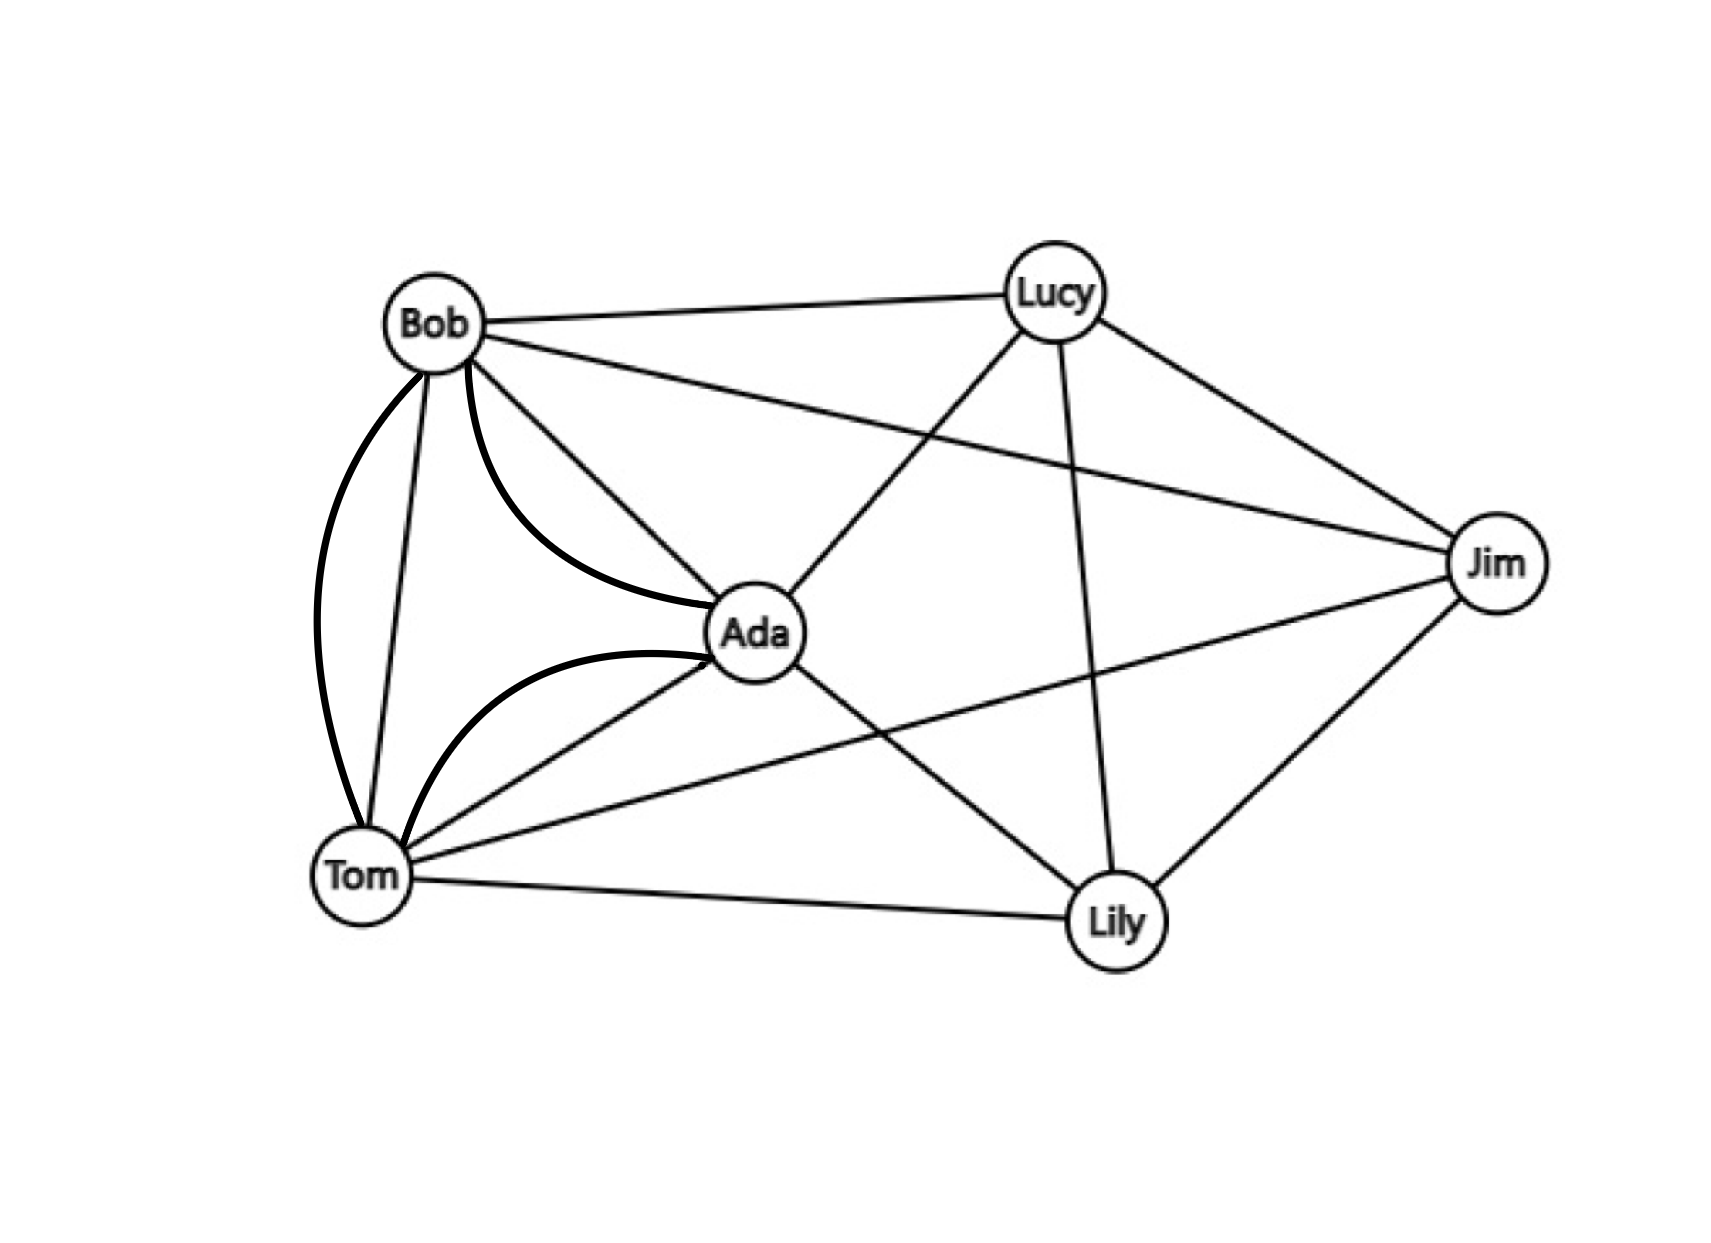
\includegraphics[width=0.8\textwidth]{assets/2.png}
    \caption{3-Anonymous Graph}
\end{figure}
\newpage
the degree sequence of the graph is $\{6, 6, 6, 4, 4, 4\}$ which is 3-anonymous.

\subsection{(c)}
In section (a), the information loss is:
\begin{equation}
    \begin{aligned}
        L(G, G') & = 1 - \frac{|\Delta(E, E')|}{\max(|E|, |E'|)} \\
                 & = 1 - \frac{8}{9} = \frac{1}{9}
    \end{aligned}
\end{equation}
In section (b), the information loss is:
\begin{equation}
    \begin{aligned}
        L(G, G') & = 1 - \frac{|\Delta(E, E')|}{\max(|E|, |E'|)} \\
                 & = 1 - \frac{8}{15} = \frac{7}{15}
    \end{aligned}
\end{equation}
\end{document}